\begin{figure}[h!]
	\centering
	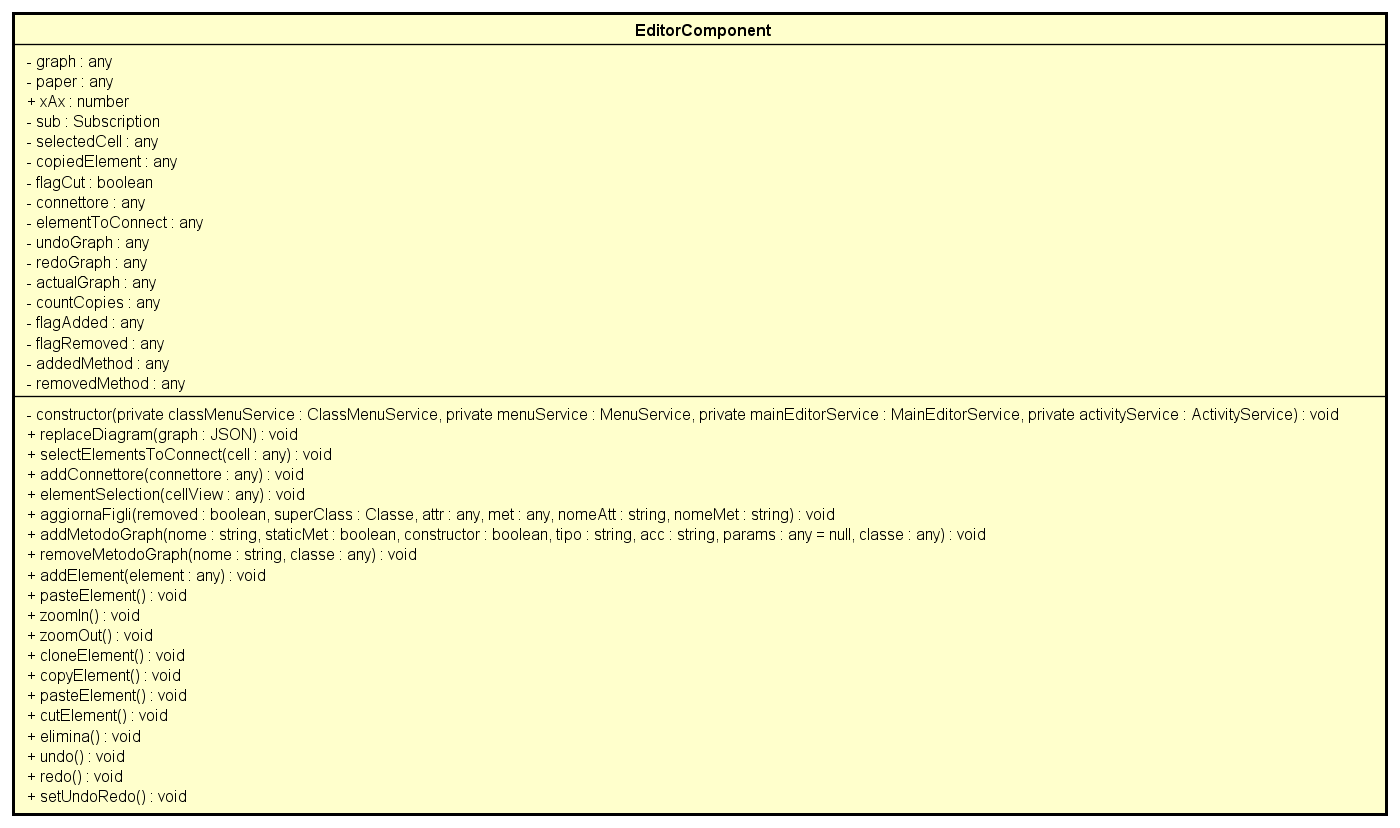
\includegraphics[scale=0.5]{res/sections/SpecificaFrontEnd/Components/Disegnetti/editor.png}
	\caption{Diagramma della classe EditorComponent}
\end{figure}

\begin{itemize}
	\item \textbf{Descrizione:}\\
	Questa classe è il componente principale di gestione dell'editor.
	\item \textbf{Utilizzo:}\\
	Viene utilizzato per la gestione dell'editor.
	\item \textbf{Attributi:}
		\begin{itemize}
			\item \emph{-graph: any}\\
            Contiene tutti gli elementi del grafico
            \item \emph{-paper: any}\\
            Assicura che vengano renderizzati gli elementi del grafico
            \item \emph{+xAx: number}\\
            Serve per scalare il grafico
            \item \emph{-sub: Subscription}\\
            Permette la funzione di zoom
            \item \emph{-selectedCell: any}\\
            Punta all'elemento selezionato con il click
            \item \emph{-copiedElement: any}\\
			Punta all'elemento copiato o tagliato
			\item \emph{-flagCut: boolean}\\
			Indica se l'elemento è stato tagliato, altrimenti è stato copiato
            \item \emph{-connettore: any}\\
            Il tipo del connettore selezionato
            \item \emph{-elementToConnect: any}\\
            Punta all'elemento selezionato con il click, che sarà collegato con il connettore
			\item \emph{-undoGraph: any}\\
			Punta al grafico dopo aver annullato l'ultima operazione
			\item \emph{-redoGraph: any}\\
			Punta al grafico dopo aver ripristinato l'ultima operazione annullata
			\item \emph{-actualGraph: any}\\
			Punta al grafico attuale
			\item \emph{-countCopies: any}\\
			Conta il numero di copie dello stesso elemento
			\item \emph{-flagAdded: any}\\
			Indica se bisogna ascoltare l'evento aggiungere del grafo
			\item \emph{-flagRemoved:any}\\
			Indica se bisogna ascoltare l'evento rimuovere del grafo
			\item \emph{-addedMethod: any}\\
			Indica al metodo annulla se un metodo è stato aggiunto
			\item \emph{-removedMethod: any}\\
			Indica al metodo annulla se un metodo è stato rimosso
		\end{itemize}
	\item \textbf{Metodi:}
		\begin{itemize}
			\item \emph{-constructor(private classMenuService: ClassMenuService, private menuService: MenuService, private mainEditorService: MainEditorService, private activityService: ActivityService)}\\
    		Costruttore della classe\\
    		\textbf{Parametri:}
    		\begin{itemize}
    			\item \emph{classMenuService: ClassMenuService}\\
    			Crea un istanziazione di ClassMenuService
    			\item \emph{menuService: MenuService}\\
    			Crea un istanziazione di MenuService
    			\item \emph{mainEditorService: MainEditorService}\\
    			Crea un istanziazione di MainEditorService
    			\item \emph{activityService: ActivityService}\\
    			Crea un istanziazione di ActivityService
    		\end{itemize}
    		\item \emph{+replaceDiagram(graph: JSON)}\\
    		Rimpiazza l'editor con una nuova finestra contenuta nel file JSON\\
    		\textbf{Parametri:}
    		\begin{itemize}
    			\item \emph{graph: JSON}\\
    			File contenente la finestra
    		\end{itemize}
    		\item \emph{+selectElementsToConnect(cell: any)}\\
    		Seleziona gli elementi da collegare con il connettore\\
    		\textbf{Parametri:}
    		\begin{itemize}
    			\item \emph{cell: any}\\
    			Elemento da collegare
    		\end{itemize}
    		\item \emph{+addConnettore(connettore: any)}\\
    		Aggiunge un connettore alla classe\\
    		\textbf{Parametri:}
    		\begin{itemize}
    			\item \emph{connettore: any}\\
    			Connettore da aggiungere
    		\end{itemize}
    		\item \emph{+elementSelection(cellView: any)}\\
    		Seleziona una shape nell'editor\\
    		\textbf{Parametri:}
    		\begin{itemize}
    			\item \emph{cellView: any}\\
    			Shape da selezionare
    		\end{itemize}
    		\item \emph{+aggiornaFigli(removed: boolean, superClass: Classe, attr: any, met: any, nomeAtt: string, nomeMet: string)}\\
    		Aggiorna i metodi e gli attributi figli della classe padre\\
    		\textbf{Parametri:}
    		\begin{itemize}
    			\item \emph{removed: boolean}\\
    			Indica se deve rimuovere un attributo o un metodo
    			\item \emph{superClass: Classe}\\
    			Classe padre
    			\item \emph{attr: any}\\
    			Attributo da aggiungere
    			\item \emph{met: any}\\
    			Metodo da aggiungere
    			\item \emph{nomeAtt: string}\\
    			Attributo da rimuovere
    			\item \emph{nomeMet: string}\\
    			Metodo da rimuovere
    		\end{itemize}
    		\item \emph{+addMetodoGraph(nome: string, staticMet: boolean, constructor: boolean,
    tipo: string, acc: string, params: any = null, classe: any)}\\
    		Aggiunge alla cella class un metodo\\
    		\textbf{Parametri:}
    		\begin{itemize}
    			\item \emph{nome: string}\\
    			Nome del metodo
    			\item \emph{staticMet: boolean}\\
    			True se è marcato static
    			\item \emph{constructor: boolean}\\
    			True se è un costruttore
    			\item \emph{tipo: string}\\
    			Tipo di ritorno del metodo
    			\item \emph{acc: string}\\
    			Accessibilità del metodo
    			\item \emph{params: any}\\
    			Lista dei parametri del metodo
    			\item \emph{classe: any}\\
    			Indica la cella
    		\end{itemize}
    		\item \emph{+removeMetodoGraph(nome: string, classe: any)}\\
    		Rimuove un metodo dalla cella classe\\
    		\textbf{Parametri:}
    		\begin{itemize}
    			\item \emph{nome: string}\\
    			Nome del metodo
    			\item \emph{classe: any}\\
    			Indica la cella
    		\end{itemize}
    		\item \emph{+addElement(element: any)}\\
    		Aggiunge un elemento all'editor\\
    		\textbf{Parametri:}
    		\begin{itemize}
    			\item \emph{element: any}\\
    			Elemento da aggiungere
    		\end{itemize}
    		\item \emph{+pasteElement()}\\
    		Incolla un elemento precedentemente copiato
    		\item \emph{+zoomIn()}\\
    		Effettua lo zoom in avanti
    		\item \emph{+zoomOut()}\\
    		Effettua lo zoom all'indietro
    		\item \emph{+cloneElement()}\\
    		Clona l'elemento selezionato
    		\item \emph{+copyElement()}\\
    		Copia l'elemento selezionato
    		\item \emph{+pasteElement()}\\
    		Incolla l'elemento precedentemente copiato/tagliato
    		\item \emph{+cutElement()}\\
    		Taglia l'elemento selezionato
    		\item \emph{+elimina()}\\
    		Elimina l'elemento selezionato
    		\item \emph{+undo()}\\
    		Annulla l'ultima azione
    		\item \emph{+redo()}\\
    		Ripristina l'ultima azione annullata
    		\item \emph{+setUndoRedo()}\\
    		Aggiorna il diagramma attuale e il undoGraph
		\end{itemize}
\end{itemize}